% !TEX TS-program = pdflatex
% !TEX encoding = UTF-8 Unicode

% This is a simple template for a LaTeX document using the "article" class.
% See "book", "report", "letter" for other types of document.

\documentclass[11pt]{article} % use larger type; default would be 10pt

\usepackage[utf8]{inputenc} % set input encoding (not needed with XeLaTeX)

%%% Examples of Article customizations
% These packages are optional, depending whether you want the features they provide.
% See the LaTeX Companion or other references for full information.

%%% PAGE DIMENSIONS
\usepackage{geometry} % to change the page dimensions
\geometry{a4paper} % or letterpaper (US) or a5paper or....
% \geometry{margin=2in} % for example, change the margins to 2 inches all round
% \geometry{landscape} % set up the page for landscape
%   read geometry.pdf for detailed page layout information

\usepackage{graphicx} % support the \includegraphics command and options

% \usepackage[parfill]{parskip} % Activate to begin paragraphs with an empty line rather than an indent

%%% PACKAGES
\usepackage{booktabs} % for much better looking tables
\usepackage{array} % for better arrays (eg matrices) in maths
\usepackage{paralist} % very flexible & customisable lists (eg. enumerate/itemize, etc.)
\usepackage{verbatim} % adds environment for commenting out blocks of text & for better verbatim
\usepackage{subfig} % make it possible to include more than one captioned figure/table in a single float
% These packages are all incorporated in the memoir class to one degree or another...

%%% HEADERS & FOOTERS
\usepackage{fancyhdr} % This should be set AFTER setting up the page geometry
\pagestyle{fancy} % options: empty , plain , fancy
\renewcommand{\headrulewidth}{0pt} % customise the layout...
\lhead{}\chead{}\rhead{}
\lfoot{}\cfoot{\thepage}\rfoot{}

%%% SECTION TITLE APPEARANCE
\usepackage{sectsty}
\allsectionsfont{\sffamily\mdseries\upshape} % (See the fntguide.pdf for font help)
% (This matches ConTeXt defaults)

%%% ToC (table of contents) APPEARANCE
\usepackage[nottoc,notlof,notlot]{tocbibind} % Put the bibliography in the ToC
\usepackage[titles,subfigure]{tocloft} % Alter the style of the Table of Contents
\renewcommand{\cftsecfont}{\rmfamily\mdseries\upshape}
\renewcommand{\cftsecpagefont}{\rmfamily\mdseries\upshape} % No bold!

%%% END Article customizations

%%% The "real" document content comes below...

\title{An Applied Method for Synthetic Spatially Distributed Continuous Precipitation Development}
\author{Quebbeman, J.A., Carney, S., Schaeffer, M., Neff, K.}
%\date{} % Activate to display a given date or no date (if empty),
         % otherwise the current date is printed 

\begin{document}
\maketitle

\section{Introduction, Issue, and Need}

Hydrologists and engineers require continuous timeseries of hydrologic data, such as precipitation or streamflow, for a wide range of purposes. These may include reservoir operating rule development and testing, energy modeling at hydropower facilities, or risk analysis, for example. Multi-year continuous precipitation data is beneficial for use in both lumped and distributed hydrologic models, although acquiring a sufficiently long period of record can be challenging.
Periods longer than the available record are commonly needed for additional statistical support, risk evaluation, and distribution fitting, although a reliable, accurate, and rapid means of developing a synthetic series maintaining spatial and temporal correlations as observed in nature is required. Critical aspects include a) maintenance of hyetograph patterns, b) maintenance of appropriate spatial relationships between distributed precipitation locations, and c) preservation of storm seasonality.
Maintenance of hyetograph temporal patterns is critical when evaluating hydrologic events and the subsequent system responses. For example, is most of the storm depth achieved during a short duration, or is the storm intensity fairly constant over the duration of the event?  Beyond just the distribution of precipitation for a single location, is the timing of precipitation over a number of basins. Storms may ‘roll’ across large regions resulting in variable start and end-times of the precipitation event at different locations. Assuming precipitation begins for every location at a uniform time is not realistic, nor is the assumption that all areas will use identical distributions of the precipitation.
Not only is the timing and distribution of precipitation important, but so are the inter-storm periods. How many hours or days is possible between precipitation events, and is there any correlation with the proceeding event or dry period?
Precipitation can occur over many different locations, each of which with different event depths. Dominant or typical storm depths can vary significantly over large regions, especially due to factors such as orographic effects. The ‘center’ of a storm shouldn’t be randomly located across a basin, but rather, should mimic the regions of the basin with typically observed higher precipitation. Relationships for seasonal or annual precipitation totals between basins needs to be maintained, and symmetric isohyets shouldn’t be used for distributing precipitation totals.
	
\section{Existing approaches for creating synthetic series}

Synthetic generation of continuous hydrologic series, such as streamflow, is traditionally completed using Autoregressive Moving Average (ARMA) techniques \cite{Salas1980}, although an alternative streamflow resampling approach using bootstrapping with k-nearest neighbors has been developed \cite{Lall1996}, demonstrating the power of resampling or bootstrapping techniques \cite{Efron1998} in hydrologic applications. This can be extremely important for bi-modal distributions, which are not well captured using ARMA techniques.

The Markov renewal process is commonly used, where precipitation at the current step is only dependent on the previous step, but again, is not spatially correlated between sites or locations \cite{Foufoula-Georgiou1987}. A technique for bootstrap sampling daily meteorological variables conditioned on the previous days states as a 1-step Markov process was developed \cite{Rajagopalan1999}, although this was only completed at a single location, rather than allowing for multi-site spatially correlated sampling.

Wilks developed a sampling procedure for precipitation at multiple sites that are serially independent with time, but spatially correlated (Wilks, 1998), and was later extended to include temperature sampling procedures (Wilks, 1999). This procedure works well for temporal series that are spatially correlated but serially independent, or have limited Markov correlations, but does not perform well for higher temporal and spatial resolution of storm events (e.g. 1-hour or 6-hour precipitation generation during an extended event). 

Precipitation generation can also be completed using point-process models, such as using the Neyman-Scott rectangular pulses model \cite{Rod-Iturbe1987}, although spatial multi-site correlation is not addressed.

Shorter temporal resolution synthetic generation was proposed by Bardossy using a simulated-annealing approach with a Metropolis-Hastings sampling algorithm \cite{Bardossy1998}. In this case, short temporal precipitation series could be constructed, although the approach does not scale well to distributed or multi-site generation. This approach was later extended as a multi-site and multi-variable weather process \cite{Buishand2001} using k-nearest neighbors. This approach allows for the generation of extreme and unobserved event sequences, the major goal of synthetic generation, although a tendency to under standard deviations and autocorrelation coefficients of precipitation and temperature was observed. 

Simple resampling of the historic record may create a unique sequence of events, but the goal is creation of a unique events beyond those observed in the historic record. This should occur in both short temporal periods (e.g. 1-hour intensities), but also aggregated into longer periods (e.g. monthly total precipitation depths). Resampling of observed historic record may help on the latter goal, but will not be able to address the former goal. Scaling of the observed record will create extreme events, but causes significant skew and bias in the statistics of the series.

Further, many powerful synthetic generation techniques are available for point-processes, but an approach is needed that maintains spatial, temporal, and seasonal statistics of precipitation without biasing the data.

Here, we outline an approach using an event-based alternating renewal bootstrap resampling and scaling approach, which helps to address these issues in creating continuous long-term synthetic records of precipitation.

\section{Approach to Address Issue}

The approach developed here uses bootstrapped ‘events’ covering a distributed region, therefore, the available observed record needs to be divided into discrete periods of WET and DRY. The definition of DRY periods is fairly straight-forward - contiguous periods without precipitation across the entire region of interest (e.g. given subbasins, or a gridded region). A WET period consists of timesteps when any part of the region of interest experiences precipitation, although in this case, a threshold depth and duration is required to be exceeded for the step to be considered an ‘event’.

For example, a 1-hr timestep interval may apply a minimum 1/10th of inch threshold which must be exceeded before the timestep is considered WET. Each timestep in the available period of record is designated as either WET or DRY. Note, all locations are labeled as either WET or DRY for any given timestep, as long as somewhere in the region of interest experienced precipitation above the threshold. These periods are then aggregated with unique event labels for contiguous periods. The duration of the WET and DRY periods (not the same as the timestep duration) will change between events. 

A sample table showing the transition from wet to dry (last row) using 6-hour interval data with a unique identifier (Groups) is shown in Table XXX. Here, a WET step is denoted with Rain=1, whereas DRY denotes Rain=0. All contiguous timesteps with a Group identifier of 1.1 are considered part of a single WET event, and 2.0 is the start of timesteps denoting a contiguous period of DRY. The next WET event would be labeled as 2.1, and so forth.
 
Table 1- Example Timestep Categorization and Event Grouping Table
Similarly, a sample of this process is also shown in Figure XXX, which displays the breaks between WET and DRY periods for the month of June in 1989 for a sample watershed, with precipitation hyetographs for all subbasins shown for over the basin of interest.
 
Figure 1 – Sample Division of WET (Rain somewhere in the area of interest) and DRY Periods
For any given WET period, the entire temporal series of precipitation is known at all points over the given event duration. In many cases, an event for the region of interest may only actually result in precipitation over a limited portion of the basin; not all areas or subbasins need to receive precipitation for a temporal period to be considered a WET step.

This process is repeated for the entire available record, ideally over many years and decades of records, resulting in thousands of unique alternating WET and DRY period event groups. The next step is to determine and record any seasonal information that may be relevant. Typically, the types of storms, magnitudes, locations, durations, etc. vary over seasons. Therefore, seasonality needs to be addressed and recorded with each unique event identifier. This could occur in annual quarters or months, for example. Data should be reviewed to identify varying seasonal event properties and relevant temporal length scales, although a month is typically acceptable. Groups of events overlap month calendar breaks or other predefined intervals, whereas each event needs to be assigned to a single period. This can be achieved by evaluating the median season period experienced by the event, and assigning it to the entire event even with period overlap.

With a record of unique events, the total mean aerial event depth needs to be determined. For a lumped model approach, this is completed using a weighted-area approach to estimate the mean storm depth ($\hat P$),
%P ̂=∑_(i=1)^N▒∑_t^T▒P_(i,t) /A_i  

where N is the number of event-wetted subbasins (or gridded cells), A is the area of each subbasin (or cell), and $P_{i,t}$ is the precipitation in subbasin i at timestep t, through total event duration T. 

Grouped by the associated season (e.g. monthly), distributions of WET event depths are fitted to appropriate distributions. Again, this will change by region and the most appropriate distribution, especially with respect to extreme values, should be chosen. The authors have good experience with a Mixed Exponential distribution (Hundecha, et al., 2009). The probability density function (PDF) can be expressed as,

\begin{equation}
f(x)=\alpha\times\lambda_1 \exp(-\lambda_1 (x-x_1))+(1-\alpha)\times\lambda_2 \exp(-\lambda_2 (x-x_2))
\end{equation}
where $\lambda_i ,\in(1,2)$ is the inverse of the mean, and $\alpha$ is a weighting factor between the two exponential distributions, and $x_i$ is a location parameter.

Each month was parameterized separately (five parameters) using a numerical approach minimizing the error between the model cumulative distribution function and the observed empirical distribution function (EDF). 

The storm depths for each month can be compared to the fitted monthly distributions using Cunnane probability plotting positions (Cunnane, 1978) and an Extreme Value Type I probability plotting scale (Santner1973), as shown in Figure XXX using sample data. 

 
Figure 2 - Monthly Non-Exceedance Comparisons between Observed Data and Fitted Models
For most months, the distribution fits the data extremely well on both low and high-levels of non-exceedance. A few exceptions include March where low depth events are over estimated, and high-depth events are slightly under-estimated. August is notable on the high-depth end of the distribution, where the model is over-estimating depths. All of the distributions are considered acceptable, and are expected to project accurately monthly depths beyond those observed in the historical record.

The process of creating a synthetic record uses an alternating renewal process between the defined collections of WET and DRY events, sequentially appended to the set. The start of a new period, be it DRY or WET, uses the seasonal period (i.e. month) distributions for total event precipitation, samples from storm templates for that given period, and uses the dry-period sampling from the historical record. This process is repeated until the desired bootstrapped period length is achieved, possibly requiring truncation at the end of the series if the length is beyond the desired record length.

\section{Event Sampling}

For a given seasonal block (e.g. months), all years of data are aggregated for distribution fitting, although further division beyond seasonal aggregation for all years may be warranted, such as accounting for longer-term processes (e.g. PDO, El Nino, etc.). In this case, supplemental period identification may be needed, such as ‘dry year’, ‘wet year’, ‘normal year’, in addition to the intra-annual definitions already established. 

With these periods fully identified and labeled seasonally, and distributions are fit to each unique combination, storm depth samples can be drawn randomly. Closed form analytical solutions for inverted CDFs are not possible, thus samples were obtained numerically. A random uniform U[0,1] representing the CDF density was sampled. Then, values of depths on the mixed Exponential CDF are iterated until the calculated CDF value matches the sampled CDF value.

The advantage of using fitted distributions rather than using only observed storm depths is clearly the ability to create event depths greater than those observed in the historic record; bootstrapping only observed depths would lead to a gross underestimation in the frequency of larger events. In constructing a new hydrologic series, sampling from these fitted seasonal (and possibly inter-annual) depth distributions will match the statistics of the observed record, but allow extension to larger and unobserved precipitation events and unique sequences.

Sampling of DRY periods is simply completed by randomly drawing from the collection of events grouped into a given seasonal block. Although distributions of the dry-period duration could be fit and sampled similarly to total precipitation event depths, the available record and diversity for dry-period event durations was deemed sufficient. 

One potential concern is the ability to sample storm depths, storm templates (durations), and dry durations, randomly without concern for event persistence. All three of these metrics need to be evaluated at the appropriate seasonal pattern with an Autocorrelation Function (ACF) to determine if serially independent sampling is possible. 

\section{Storm Template Selection}

Once a depth has been sampled from the distribution, an observed historic event can be scaled such that the total aerial depth matches that of the random sample. Using historic event storm templates (contiguous WET periods, which have a unique Group ID) has several advantages, including the maintenance of both the temporal and spatial patterns as observed in nature. Further, complicated hyetographs are realistically represented, compared to generalized hyetograph forms, such as those used in the NRCS or HMR-52 methods, for example.

Selection of an appropriate WET template is critical, where all events are not equally likely for a given sampled depth. For example, a twelve inch storm event is not likely to occur over a 1-hour period, whereas a 72-hour period is more likely. To select an appropriate template, the labeled events are sorted by total event depth. The sampled depth is then located within the observed sorted depth series, and a uniform density function is used to randomly sample an event from the nearest ten events. If a sample is drawn greater than the observed record, for example, then the top 10 largest storms will be used to randomly select a template. This template event is scaled to the sampled depth, which retains the spatial and temporal variation of the original event.

	Continuous Series Construction
Once a given WET period (DRY period) is sampled, an alternating DRY period (WET period) is then sampled and appended to the end of the series, following the alternating renewal method. The corresponding distributions used for sampling, or collections of templates and DRY periods, depend on the starting date of the event and the corresponding seasonal period. Repeating this process many thousands of times allows for the creation of a unique precipitation sequence. If required, the last event is truncated to meet the desired series length.

\section{Case Study}

This process was used to develop 1000-years of synthetic data (years 2000 through 2999) for the Tennessee Valley Authority (TVA) watershed. This drainage area covers XXX sq. miles, divided into 126 subbasins. Available Mean Aerial Precipitation (MAP) data from a period of January, 1950 to May of 2013 was available for the entire region, and was processed using this approach, resulting in over 326,000 unique WET and DRY events. These periods were assigned the appropriate month of the year for separation by season. Long-term processes, such as sustained droughts, longer-term persistent wet-seasons, and climatic trends were not included in this process.
The resulting 1000-year bootstrapped series is used for initial state sampling within the Stochastic Event Flood Model (SEFM) approach. This risk-based analysis of the TVA system requires both extreme precipitation events to be evaluated, but also extreme initial conditions, warranting the development of this long-term bootstrapped series for extreme initial condition sampling beyond those observed in the historic record. 
After creating unique WET and DRY events from the nearly 63-years of MAP data, the properties of the series were evaluated for consistency with the required assumptions for sampling. Autocorrelations were checked of the dry period durations, storm event depths, and storm event durations. In all cases, the events were serially independent, with two months being an exception. 

The exception months were October and November, where the Ljung-Box test indicated a significant autocorrelation (p-value<0.05) for total storm depth and duration, indicating some degree of persistence at short lags. This persistence is recognized, but considering it is not for all months, nor is the significance much less than a p-value of 0.05, serial independence sampling was retained. Further, this correlation was negative, indicating shorter or smaller events after a larger event. From a flood and high flow perspective, the focus of the study for TVA, a lag-1 negative autocorrelation is less concerning than compared to a significant positive correlation, where significant events are leading to subsequent significant events.

 \begin{figure}%[htbp]%
\center
\noindent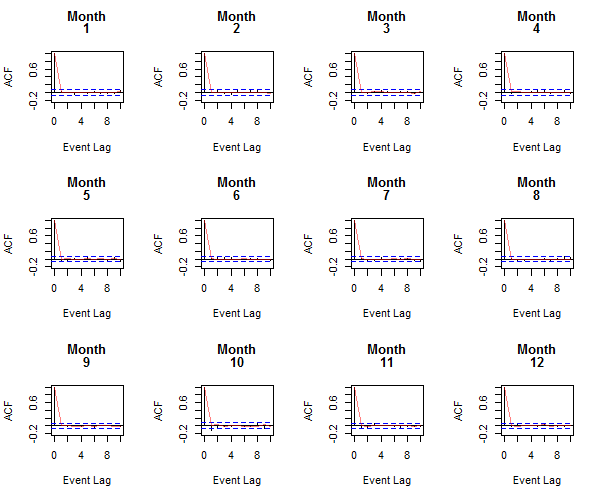
\includegraphics[scale=.7]{./Figures/ACF_Monthly_Totals} 
\caption[]{Monthly ACF Values for Event Precipitation Totals}
\label{MonthlyACFTotal}	
\end{figure}

With a developed bootstrapped series, a number of diagnostic tests were completed to ensure the synthetic series matches the properties of the observed series, even with events greater than those observed in the record. Several important tests include:

	Annual and Monthly histograms of event totals, durations, and dry-durations,
	Evaluation of extreme event frequencies against fitted monthly distributions,
	Evaluation of subcatchment total precipitation ensuring greater wet-periods than those observed historically.

Figure XXX shows a sample of several statistics comparing the observed to the bootstrapped record for the month of September. Note the bimodal histogram replicated in the series for rain event duration, in addition to the fit of intensity, total and dry event duration. It’s worth noting that the bootstrapped series is under estimating the frequency of small precipitation event totals compared to the observed record, which is in-line with the fitted monthly frequency distributions. In all months, there is no significant difference between the observed and bootstrapped event empirical distribution functions.

\begin{figure}%[htbp]%
\center
\noindent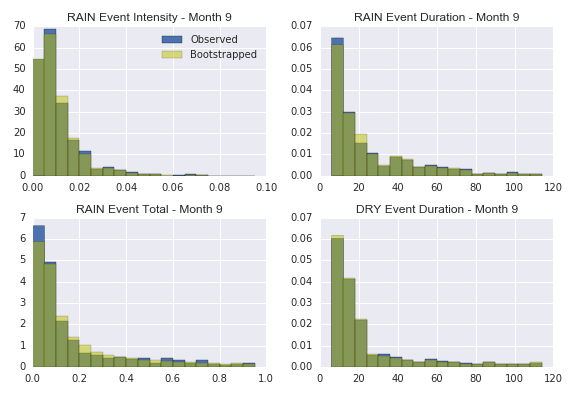
\includegraphics[scale=.7]{./Figures/Hist_DF_Comparison_Month9} 
\caption[]{Histogram comparison of observed and synthetic data for September}
\label{HistogramPost}	
\end{figure}

As noted earlier, autocorrelation of sampled events was not deemed significant, and thus tests for replicating observed autocorrelation are not included here.

Finally, the process should result in an improved diversity of extreme events and months. The goal of this process is to create longer-term series with exceptionally wet and dry periods. Figure XXX shows the maximum monthly total precipitation for each of the subcatchments between the original historic series, and the bootstrapped series. As expected, the bootstrapped creates, at some point in the record, significantly larger monthly precipitation totals, denoting a successful extrapolation of the historic record to unobserved series.

 \begin{figure}%[htbp]%
 \center
\noindent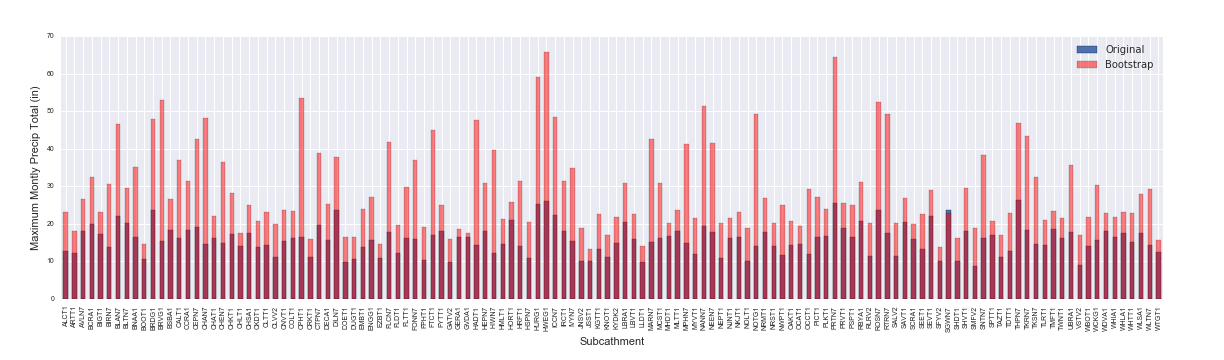
\includegraphics[scale=.5]{./Figures/Monthly_Max_Prec3} 
\caption[Maximum Monthly Precipitation Total for both the observed and synthetic record for each subcatchment]
{Maximum Monthly Precipitation Total for both the observed and synthetic record for each subcatchment}
\label{MaxMonthly}	
\end{figure}

\section{Discussion and Conclusions}

One key assumption to this process is the assumption of parameter stationarity; clearly, 1000-year period in the current climatic regime would experience variations of precipitation event totals and patterns. This is ignored in this process, as the need for the long-term dataset is in stochastic sampling, rather than needing to understand a complete and contiguous 1000-year period.

Similarly, patterns of sustained single or multi-year dry or wet-periods is also ignored. The distributions are assumed to cover the range of wet and dry years without explicit categorization or conditional sampling. This could potentially be added through additional classification, but has been ignored for this application.

Although this model was applied to a lumped hydrologic model utilizing subcatchments, there is nothing prohibiting the application of this process to a distributed hydrologic model. In this case, variable thresholds for breaking between WET and DRY periods may need to be tested (e.g. depth of event in addition to minimum number of cells experiencing precipitation), but it can easily be extended to a distributed system.

This process allowed for the development of both spatially and temporally long-term correlated precipitation data. Histograms of the storm event seasonal properties in addition to dry periods are maintained with the required correlations, while diversity to the storm events is added through a distribution fitting and sampling approach. This process allowed the easy development of 1000-years of synthetic data for advanced hydrologic modeling applications and sampling.

\section{Acknowledgements}

This work was generously supported by the Tennessee Valley Authority (TVA) under contract with Riverside Technology, inc. (\#1364). 

\bibliographystyle{plain}
\bibliography{Riverside}



\end{document}
